\documentclass[a4paper]{article}
\usepackage[hmargin=1in, vmargin=1in]{geometry}
\usepackage{makeidx}
\usepackage{fancyhdr}
\pagestyle{fancy}
\usepackage[pdftex]{graphicx}
\usepackage{amsmath}
\usepackage{listings}
\makeindex
\begin{document}
\begin{center}
\title{Three dimensional coordinates into two dimensional coordinates transformation}\\
\author{Edward Gerhold}
\city{Berlin, Germany}
\date{\today}
\maketitle

Version 0.2.9 (the is getting expanded version has a few new unshaped subsections)\\

\textbf{Remark} This text may contain miscounts and logical errors (the pseudo basis term
is removed), \emph{typos},
unclear phrases, remarks, during development. But this document is living and being edited.
It is evolving from a transformation, to a documentation of the transformation plus a study
of the spaces beetween which the transformation happens and how. 

}\\

\end{center} 


\tableofcontents\\

\section{Introduction}

On a piece of paper you see three coordinate axes pointing into three
directions in space. In reality these vectors are two dimensional. Because
they point into three directions on the paper, and not into the real space.\\

\begin{figure}[ht]
\label{ijksystem}
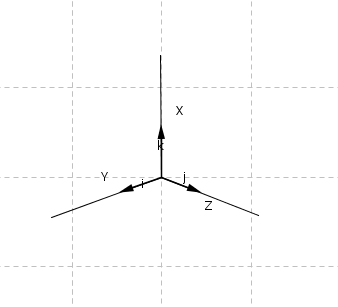
\includegraphics[scale=2]{ijksystem.png}\\
\caption{Picture of a right handed 3-D coordinate system with ijk-basis-vectors on the axes pointing
into three dimensions. See \cite{Corral1} for introduction.}
\end{figure}

In this document we will design a $\mathbb{R^{2x3}}$ basis for the coordinate transformation. 
A basis is multiplied with the values of the coordinates to move for each component 
a piece, to end the move on the correct new point.
In the case of cosines and sines, we move left and right and up and down, to 
tell you directly, what happens, when we multiply the coordinates with the matrix.\\

\textbf{What we will do in the document}

\begin{enumerate}
\item Choose angles for our coordinate axes around the unit circle to lay out three axes.
\item Write down the basis vectors for each coordinate axis
\item Assemble a matrix with the vector basis for a point by point transformation.
\item Read the example source code for a computer function, which is exactly two lines long. One for the new $x$ and one for the new $y$.
\item Derive the generic case of transforming coordinate systems down to the plane.
\end{enumerate}

\section{Designing a $R^{2x3}$ basis for our transformation from $R^{3}$ to $R^{2}$}

\subsection{The $_{n}$ index for $_x,_y,_z$ with $_x=1$, $_y=2$ and $_z=3$}

The index $_{n}$ in $r_{n}$, $\varphi_{n}$, $\vec{e}_{n}$ is the index for $_x$,$_y$,$_z$. For example $\varphi_{n}$  stands $\varphi_x, \varphi_y, \varphi_z$. $r_{n}$ stands for $r_x$, $r_y$ and $r_z$. $\vec{e}_{n}$ is for $\vec{e}_x$, $\vec{e}_y$, $\vec{e}_z$ It is possible, that in the formulas $x,y,z$ and $1,2,3$ may be used interchangeably. For example, when summing up the products of the coordinate components with the basis components, this happens. The formula is $\sum_{i=1}^{3}\vec{x}_{i}\vec{e}_{i}$, which is a sum of $x,y,z$ and the $\cos \varphi_{n}$ terms in the first components of $\vec{e}_{n}$ for $x'$ and a sum of $x,y,z$ and the $\sin \varphi_{n}$ terms in the seconds components of $\vec{e}_{n}$ for $y'$.

\subsection{$\varphi_{n}$ the angles for the coordinate axes}

Why do we need angles? May be the first question. My answer is, we will arrange the basis vectors,
easily around a circle, by their angle. Since they are two dimensionsal. The circle is available in two dimensions.
With the arrangement around a circle, we get the right numbers, same lengths, instead of guessing wild numbers.\\

First draw three axes of a 3-D coordinate system on a piece of paper. Draw the horizontal x-Axis through the origin of the drawn coordinate system. You could directly add the y-axis, to see a 2-D coordinate system carrying your two dimensional 3-D system. A system with three vectors pointing into three directions, originating in the origin of the real R^2 space.\\

\begin{figure}[ht]

\includegraphics{handsystems.png}
\caption{A left-handed and a right handed coordinate system. They just have different angles in our 2-D projection.}
\end{figure}

Each of the three vectors has an angle, counted from the horizontal positive x-axis, going counterclockwise around the origin. The
angle between the axes themselves isn´t what we want. We want the angle beginning on the real 2-D x-axis, to feed the cos and sin functions with, when calculating the real numbers of each basis vector.\\

In this document, i will call the angles $\angle \varphi_{n}$ or just $\varphi_{n}$. If they are measured in degrees or radians depends
on the cosine and sine functions you use. And on how you would like to read your own definition.

Let $\varphi_{n}$ be the set of axis angles, one for each axis. I put them into a set in this document to simplify the access by
using the index $_{n}$ together with $_x, _y, _z$ or $1,2,3$. $\varphi_x$ or $\varphi_1$ is the angle of the x-axis. $\varphi_y$ or $\varphi_2$ is the angle of the x-axis and $\varphi_z$ or $\varphi_3$ is the angle of the x-axis. 


\begin{displaymath}
\varphi_{n} := \{\varphi_x, \varphi_y, \varphi_z\} = \{ \varphi_1, \varphi_2, \varphi_3 \}
\end{displaymath}

We will need the three angles for the axes shortly. So don´t forget it over the next lines.


\subsubsection{Degrees or radians?}

Depending on the cosine and sine functions and the input value for the angles, you may have to convert the degrees to radians, or
the other way round, the radians to degrees. For example, the JavaScript Math.cos and Math.sin functions take the values in radians.\\

\begin{example}
\textbf{example}
The function rad converts degrees to radians, it´s useful for computer functions taking radians.
\begin{displaymath}
\text{rad}(\phi) := \frac{\pi}{180} \times \phi, \phi \in \mathbb{R}
\end{displaymath}


Here is an example of three angles. The three axes have an angle of 120 degrees between each. But since we start counting counterclockwise and from the real horizontal axis of the plane, the angles are 210, 330, 90 in degrees, respectivly. And
because of the cosine and sine functions taking radians, we convert the values to radians.
 
\begin{displaymath}
\varphi_x = \text{rad(210)}, \varphi_y = \text{rad(330)}, \varphi_z = \text{rad(90)}
\end{displaymath}

\begin{displaymath}
\varphi_x &= \frac{\pi}{180} \times 210 &= \frac{7\pi}{6},  
\varphi_y &= \frac{\pi}{180} \times 330 &= \frac{11\pi}{6}, 
\varphi_z &= \frac{\pi}{180} \times 90 &= \frac{\pi}{2} 
\end{displaymath}
\end{example}

\textbf{example}
The function deg converts the other way round and from radians to degrees. You multiply your value with the reciprocal of PI/180, namely 180/PI and get the other way round.
\begin{displaymath}
\text{deg}(\phi) := \frac{180}{\pi} \times \phi, \phi \in \mathbb{R}
\end{displaymath}

If you would like to get hands on angles, cosines, sines, or need a refresher, \cite{Corral2} is a good choice. But also \cite{Corral1} and \cite{Strang2} bring unit circles, polar coordinates, sines, cosines and more informations.

\subsection{$r_{n}$ is the length of the unit on each axis}

Before i show you the three vectors, and how to use them, we have to clear another piece of information belonging to each
basis vector. In this document it is called $r_{n}$. The r is from radius. And it stands for the length of the basis vector.
The length of the basis vector defines, how far a point in this direction will go by one unit.\\

The $r$ originates from radius from the unit circle and from the parametrization of (x,y) via cosine and sine. 
In polar coordinates the cosine and sine are multiplied with r. Also to change the length of the hypotenuse, 
the vector $\vec{r}$, which is the third side to a triangle by cosine, sine and r. 
If r is left away, the length of the basis vector is 1. Or in other words, the distance $d((0,0),(x,y))$ from the origin to $(x,y)=($$r \cos \varphi$$, $$r \sin \varphi$$)$ is $1$, if $r=1$ or if r is left away completely.\\

Pay attention to this point now, to keep the affine transformation, especially under rotation, correct. You should give all three
axes the same r-value. I will define them in this document as $r_{n}$ with one $r_x, r_y$ and $r_z$ for each coordinate axis,
to keep it complete. But if you would like to change the units on your objects, i have to recommend, that you apply a local
3x3 basis with the disjoint unit lengths. This will keep the rotation correct. In the other case, the object would suddenly
stretch the head, if you rotate it to the side, where the unit for example is longer.\\

So for the coordinate system, the best setting is $r_x = r_y = r_z$. Keeping them equal, you can rotate it realistic. But you
don´t need to keep the unit length of 1 for the vector. Elonginating the units on the axes make zooming transformations very
easy.\\

\subsubsection{Taking the norm of $\vec{e}_n$ to obtain $r_n$}

If you have some existing basis and you would like to figure out, how long r is, you can go the other way round and take the
norm of the vector. Taking the norm means to measure the length of the vector. This is done with the euclidean norm, or the
2-norm for regular purposes.\\

$r_{n} = \sqrt{\vec{e}_{n}\cdot\vec{e}_{n}}$ = $\sqrt{(\vec{e}_{n},\vec{e}_{n})}$ = $\left(\Sigma_{i=1}^{2} \vec{e}_{i}^2\right)^{\frac{1}{2}}$ = $\|\vec{e}_{n}\|$\\itt

With this formula you can not only measure the length of the basis vectors, but any vector in the $R^{3}$ and the $R^{2}$ space. 
More advanced measurements include the p-Norm, which is $\sqrt[p]{\sum_{i=1}^{n}|\vec{x}_{i}|^{p}} 1 \leq p \leq \infty$ and $\sup_{i=1..n} |\vec{x}_{i}|$ for $p=\infty}$ and the max-Norm $\|\vec{x}\|_{\infty}$= $\sup_{} \{|\vec{x}_{i}| \}$. There are matrix norms like $\|A\| = \max_{i=1..m} \sum_{j=1}^{n}A_{ij}$, which for example yields the largest row of a m by n matrix. Norms are used everywhere ing mathematics for measuring the lenghts of the vectors and matrices. And the distance function $d(\vec{x},\vec{y}) = \|\vec{x}-\vec{y}\|$ is used to measure the distance between to points or two vector tips. A vector space V with a distance function $d(x,y)=\|x-y\|$. 
  is called a metric space $(V,d)$. And a complete metric space with a norm, written $(V, \|\cdot\|)$, is a Banach space. 

A vector can be normalized to give $\|\vec{x}\| = 1$, by dividing the vector components by the length, say $\vec{w}_{normalized} = \frac{\vec{w}}{\|\vec{w}\|}$. See the appendix for more on norms and for example for a proof of the normalization.

\subsection{$\vec{e}_{n}$ are the three 2-D basis vectors}

We have drawn some axes on a piece of paper and taken the angles starting from zero counterclockwise on the x-axis.\\

Now we will write down the three basis vectors. Each vector points from the origin exactly along the first unit of the together belonging axis.\\

Let $\vec{e}_{n}$ be the set of three two dimensional basis vectors. In this document and some literature and scripts,
we call them $\vec{e}_x$, $\vec{e}_y$ and $\vec{e}_z$. Another well known names for the basis vectors are $\vec{i}$, 
$\vec{j}$ or $\vec{k}$ for example. That is equal to the picture of the coordinate axes at \ref{ijksxstem} in this document.\\

The three vectors point into the three directions of the three coordinate axes. Exactly along one unit, since we are going
to define with them the length of one unit of the corresponding axis together with the positive direction of the coordinate axis.
Multiplying the 2x3 basis with the 3x1 points later results in wonderful 2x1 points. \\

\begin{displaymath}
\vec{e}_{n} := \{\vec{e}_x, \vec{e}_y, \vec{e}_z\} = \{\vec{e}_1, \vec{e}_2, \vec{e}_3\}\\
\end{displaymath} 

There we have the set for the three basis vectors. We give them the letter $e$ and a subscript for the coordinate component in the numeric order of $x=1, y=2, z=3$. To arrange these vectors we already got around the unit circle. To measure the angles, beginning on the horizontal coordinate axis or zero, until we reach the vector. The vectors point into the positive direction of the describing axis.\\

\begin{figure}[ht]
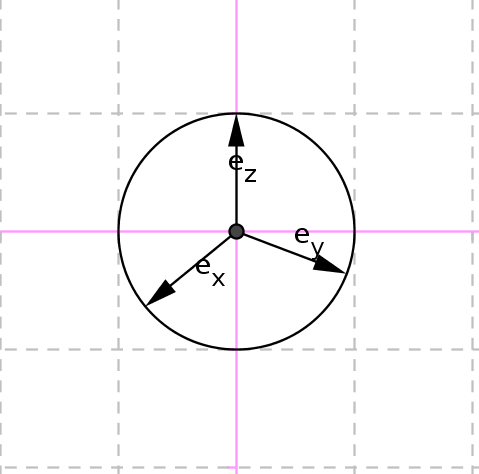
\includegraphics[scale=1]{unitvectors.png}
\caption{The three basis vectors point into the positive directions of the desired coordinate axis. They are arranged around a circle with the trigonometric functions of cosine and sine. The coordinate system shown is a righthanded coordinate system.}
\end{figure}

\begin{figure}[ht]
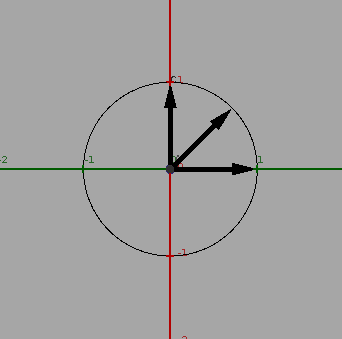
\includegraphics[scale=0.5]{lefthandbasis.png}
\caption{The three two dimensional basis vectors $\in R^{2x3}$ as a lefthanded coordinate system.}
\end{figure}


To reach all three (x,y) at the tips of the vectors, we will now pull out the cosine and sine functions and stuff them together
with $r$ and $\varphi$ into a 2x1 vector with two components. So any (x,y) on one line from the origin to far distance can be reached like in polar coordinates\footnote{Interested readers may find in \cite{Corral1}, \cite{Corral2} and \cite{Strang2} everything about polar coordinates, parametrization of x and y with cosine and sine, the unit circle and the distance or radius r and more to these topics.} with the following parametrization.\\

\begin{displaymath}
\left(\begin{array}{1}x\\y\end{array}\right) = \left(\begin{array}{1}r \cos \varphi\\ r \sin \varphi\end{array}\right)\\
\end{displaymath}\\

Which can alternativly be written like $(x,y) = (r \cos \varphi, r \sin \varphi)$.\\

Modeling the three two dimensional basis vectors with this information,
we get the following three two dimensional basis vectors. They point along the coordinate axes and are the ruler for our transformation.\\

\begin{displaymath}
\vec{e}_x := (r_x\cos(\varphi_x), r_x\sin(\varphi_x) )^T = \left(\begin{array}{1}r_x\cos(\varphi_x)\\r_x\sin(\varphi_x) \end{array}\right)\\
\end{displaymath}
\begin{displaymath}
\vec{e}_y := (r_y\cos(\varphi_y), r_y\sin(\varphi_y) )^T = \left(\begin{array}{1}r_y\cos(\varphi_y)\\r_y\sin(\varphi_y) \end{array}\right)\\
\end{displaymath}
\begin{displaymath}
\vec{e}_z := (r_z\cos(\varphi_z), r_z\sin(\varphi_z) )^T = \left(\begin{array}{1}r_z\cos(\varphi_z)\\r_z\sin(\varphi_z) \end{array}\right)\\
\end{displaymath}\\

Each component of (x,y,z) has now an own basis vector. By multiplying the cos terms for the x' and the sin terms for y' with the corresponding component of (x,y,z) and summing the three products up for each of x' and y', we directly obtain the right coordinate on the plane. All we would have to do is to connect the points again, or to fill the space between. 

\begin{figure}[ht]
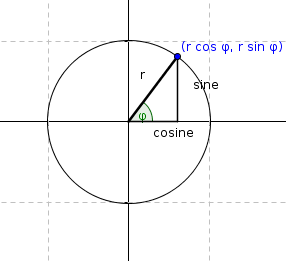
\includegraphics[scale=2]{unitcircle.png}
\caption{A picture of the unit circle, the hypotenuse r, the adjacent cosine, the opposite sine and the angle $\varphi$. It is a circle of radius r, and no longer the unit circle, if $r \neq 1$.}
\end{figure}

\subsection{About the vector basis lemma}\\

\subsubsection{The generic formula}


I am talking about multiplying the coordinates with the new vector basis, which i state to be the same as the coordinate system we drew on a piece of paper at the beginning. We wrote down the angles, made out the unit length, and wrote down the three basis vectors with the information. Where is this coming from?\\

Every mathematics, physics or related course has a lesson, where the orthogonal basis of an objects coordinate system is introduced. 
A orthogonal basis is a set of 2 or three or up to infinite orthogonal or perpendicular vectors. They describe the coordinate system, the space, the dimensions, and one has to show for excercises, that the basis is linearly independent, that each basis vector points into it´s own dimension and not into the others.\\

The one lemma we need is this general theorem for multiplying a vector with the a basis of a target coordinate system.\\

\begin{figure}
\begin{displaymath}
    \boldsymbol{E}_{\mathbb{R}^2} = \begin{pmatrix}1 & 0 \\ 0 & 1\end{pmatrix}    
\end{displaymath}
\caption{The standard basis for the $\mathbb{R^{2}}$ spans up the two dimensional space. The basis is true in $R^{2x3}$ but in $R^{2}$ just a linear combination of $\lambda\begin{pmatrix}1\\0\end{pmatrix}$ and $\mu\begin{pmatrix}0\\1\end{pmatrix}$. }
\end{figure}

The plane gives us two possible directions, to go horizontal or vertical. And in a cartesian coordinate system with infinite points, we can choose any direction around a center point (x,y). Which is in the case of our coordinate system the origin at (0,0,0) or (0,0). We will see later, that the zero vector stays in the origin fo both systems.
Any not straight move will go horizontally or vertically by componentwise amounts. Any straight move horizontally or vertically will go by one of the components only.\\


\textbf{Remark} Edward was doing it right, then wrong (wrong with his pseudo-term). The basis is correct, but the space was $R^{2x3}$. In $R^{2x3}$ the basis can be shown. In R2 it is just a linear combination of three scalars with three vectors. I will be able to formulate this out in the next versions and have nice images for explanation in mind, which i will draw for.

The point is, the general formula holds with a 2x3 basis.

The basis acts as a middler beetween the two spaces. We walk through the $R^{2x3}$ when going from $R^{3}$ to $R^{2}.$\\

In $R^{2}$ the basis is linearly dependent, and not a basis, but multiplying the coordinates with, yield the right image of the set of points processed. On the other side, in $R^{2x3}$ the basis can be explained, what i will do in the next versions. Have to read the text again, to catch my thread.\\

The formula for multiplying a vector with a base to get a new vector is this.\footnote{The formula can be found in many mathematics, chemistry and physics lecture scripts, and a good introduction is \cite{Strang1}.\\}

\begin{displaymath}
\vec{w} = \displaystyle\sum_{i=1}^{n} \vec{v}_{i}\vec{e}_{i}
\end{displaymath}

It is done componentwise for each row of the vector. $n$ is the number of the source dimensions. In our case it is $n = 3$. 
We are summing three products for each component of the new vector. Our old $\vec{v}$ is a $\vec{v} \in \mathbb{R}^3$.\\
With $\vec{v}_{i}$ as the coordinate component and $\vec{e}_{i}$ as the corresponding basis vector in the right component. 
$\vec{w}$ is the resulting new vector.  The new vector $\vec{w}$ is a $\vec{w} \in \mathbb{R}^2$.\\

In our scenario is $V \subseteq \mathbb{R^{3}}, \vec{v} \in V$ and $W \subseteq \mathbb{R^{2}}, \vec{w} \in W$.

\subsubsection{Connection to ijk-Notation}

This is also equal to

\begin{displaymath}
\vec{v} = x\vec{i} + y\vec{j} + z\vec{k}
\end{displaymath}

what also explains, what the ijk-Notation means. If you don´t use it already for determining determinants for
calculating cross products (\ref{crossproducts}). It is for describing a vector. Don´t forget, our $i, j, k$ basis is two dimensional, 
because we draw on a 2-D plane like the computer screen or a piece of paper. \\

With a 3x3 basis the vector $x\vec{i} + y\vec{j} + z\vec{k}$ is equal to \left(\begin{array}{1}x'\\y'\\z'\end{array}\right)$. But with a 2x3 basis the vector $x\vec{i} + y\vec{j} + z\vec{k}$ is becoming  \left(\begin{array}{1}x'\\y'\end{array}\right)$\\


\subsection{Time to show the operation}

The operation of multiplying the (x,y,z) coordinate with our basis vectors in order is the following:\\

\begin{displaymath}
\left(\begin{array}{1}x'\\y'\end{array}\right) = \left(\begin{array}{1}
xr_x\cos(\varphi_x) + yr_y\cos(\varphi_y) + zr_z\cos(\varphi_z)\\
xr_x\sin(\varphi_x) + yr_y\sin(\varphi_y) + zr_z\sin(\varphi_z)\end{array}\right)\\
\end{displaymath}\\

Right, this small formula brings the unexpected images of the preimage from $R^3$ to $R^2$.\\

What is new, what we know now? Each $(x,y,z)$ coordinate has to be multiplied with the vectors for the new $(x',y')$.
With the corresponding terms of the basis vectors for each of x,y,z in the matrix. That means,
to sum the products with $(x,y,z)$ and the cos terms up for $x'$ and to sum the products
of $(x,y,z)$ and the sin terms up for $y'$. This is the same as imagining walking left and
right with $\cos \varphi$ and up and down with $\sin \varphi$. Or mathematically adding positive or negative values to move up and down and left and right to the right spot. On the piece of paper, you take the ruler. You count the units, and go parallel to each axis. From the point you reached along parallel to the current axis as many units as the coordinate component has.

It is almost time to finish the matrix and to go through a set of points to draw the new set of resulting points.
For this i close the explaining chapters and come to the part of the formal mathematical definitions.\\

\section{My $\mathbb{R^{3}} \rightarrow \mathbb{R^{2}}$ transformation theorem}

Let $V$ be the set of all points $(x,y,z) \in R^3$ which are about to become transformed. $V = \{ \vec{v}=(x,y,z) | x,y,z \in R^3 \}$.
Let $W$ be the set of all points $(x',y') \in R^2$ which are the result of the transformation $W = \{ \vec{w}=(x',y') | x',y' \in R^2, (x',y')=\boldsymbol{A}\vec{v}\}$.\\

\textbf{Remark} This chapter needs to be overworked with correct definitions of the sets, domain and range, etc.\\


\subsection{The transformation matrix}
\index{Definition}
\newtheorem{Definition}{Definition}
\begin{Definition}

Let \boldsymbol{A} be the matrix containing the three, two dimensional and trigonometric, basis vectors in order, one each
column. You get a rectangular 2x3 matrix $\boldsymbol{A} \in \mathbb{R}^{2x3}: \mathbb{R}^{3} \rightarrow \mathbb{R}^{2}$. With the basis vectors $\left(\begin{array}{1}r_{n} \cos \varphi_{n}\\r_{n} \sin \varphi_{n}\end{array}\right)$ in the three columns. 

\begin{displaymath}
\boldsymbol{A} := \begin{pmatrix}
    \vec{e}_x & \vec{e}_y & \vec{e}_z
    \end{pmatrix}
    = 
    \begin{pmatrix}
    r_x\cos(\varphi_x) & r_y\cos(\varphi_y) & r_z\cos(\varphi_z) \\
    r_x\sin(\varphi_x) & r_y\sin(\varphi_y) & r_z\sin(\varphi_z) \\
    \end{pmatrix}\\
\end{displaymath}\\

$\boldsymbol{A}$ should be treated as operator $\boldsymbol{\hat{A}} \in \mathbb{R}^{2x3} : \mathbb{R}^3 \rightarrow \mathbb{R}^2$. ($\vec{x}) \mapsto \boldsymbol{A}\vec{x}$. 

\end{Definition}\\


\textbf{Remark} This chapter needs to be overworked.

\subsection{The transformation}
\index{Theorem}
\newtheorem{Theorem}{Theorem (The Fundamental Theorem of transforming 3-D Points into 2-D Points)}
\begin{Theorem}\\

If you multiply \boldsymbol{A}, the matrix of the three two-dimensional basis vectors,
with the three-coordinate point $(x,y,z)$, the result is a two coordinate point, 
$(x',y')$. This point $(x',y')$ is the correct point on the two dimensional plane,
representing the point $(x,y,z)$ from the three dimensional coordinate system, you are transforming.\\

\begin{displaymath}
\boldsymbol{A}\left(\begin{array}{1}x\\y\\z\end{array}\right) = \left(\begin{array}{1}x'\\y'\end{array}\right)
\end{displaymath}

Applying the operator \boldsymbol{\hat{A}} transforms the point $(x,y,z) \in \mathbb{R}^3$ into a new point $(x',y') \in \mathbb{R}^2$. 

\textbf{Proof}:\\

\begin{displaymath}
\boldsymbol{A}\left(\begin{array}{1}x\\y\\z\end{array}\right) = x\vec{e}_x + y\vec{e}_y + z\vec{e}_z\\
%\end{displaymath}
%\begin{displaymath}
&= \left(\begin{array}{1}xr_x\cos(\varphi_x) + yr_y\cos(\varphi_y) + zr_z\cos(\varphi_z)\\
xr_x\sin(\varphi_x) + yr_y\sin(\varphi_y) + zr_z\sin(\varphi_z)\\
\end{array}\right) = \left(\begin{array}{1}x'\\y'\end{array}\right)
\end{displaymath}

\begin{figure}[ht]
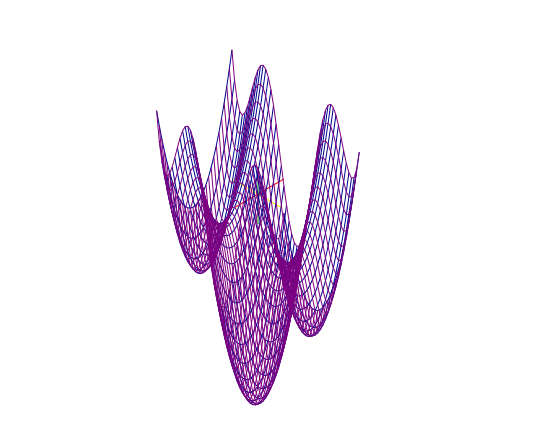
\includegraphics[scale=0.5]{fxyplot.png}
\caption{$f(x,y) = x^2 + y^2 + 3y \sin y$ from [-5,5] and [-3,3] on a Canvas2DRenderingContext}
\end{figure}


\end{Theorem}

\subsection{Computer implementations of the matrix and the transformation}
\subsubsection{Generic computer code}
\begin{example}
The following is example code for various computer systems.\\
\begin{lstlisting}
x_ = x*r*cos(alpha) + y*r*cos(beta) + z*r*cos(gamma)
y_ = x*r*sin(alpha) + y*r*sin(beta) + z*r*sin(gamma)
\end{lstlisting}
\end{example}\\


\subsubsection{JavaScript computer code}
\begin{example}
This is a full EcmaScript 6 snippet with all neccessary informations.\\
\begin{lstlisting}
let rad = (deg) => Math.PI/180*deg;
let r_x = 1, r_y = 1, r_z = 1; 
let phi_x = rad(220), phi_y = rad(330), phi_z = rad(90); 
let xAxisCos = r_x*Math.cos(phi_x), 
    yAxisCos = r_y*Math.cos(phi_y),
    zAxisCos = r_z*Math.cos(phi_z),
    xAxisSin = r_x*Math.sin(phi_x), 
    yAxisSin = r_y*Math.sin(phi_y),
    zAxisSin = r_z*Math.sin(phi_z);
let transform2d = ([x,y,z]) => [
    x*xAxisCos+ y*yAxisCos+ z*zAxisCos,
    x*xAxisSin+ y*yAxisSin+ z*zAxisSin];
let transform2dAll = (P) => P.map(transform2d);

let examplePoints = transform2dAll([[1,2,3], [3,4,5], [14,24,15]]);
\end{lstlisting}
\end{example}\\


\begin{figure}[ht]
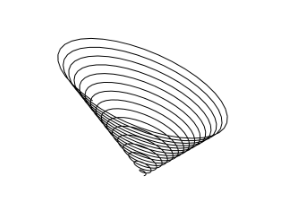
\includegraphics[scale=0.5]{conicalhelix.png}
\caption{A conical helix (t/2*Math.cos(t), t*Math.sin(t), t) shown as (x,y,z)=f(t) with implement.html on a Canvas2DRenderingContext testing the javascript example code.}
\end{figure}

\section{Corollaries}

\subsection{Converting four Dimensions down to two dimensions}\\

The theorem can be used to handle more dimensions, for example can four two-dimensional
vectors represent a 4-D space on the 2-D plane. They get converted into the correct
2-D points. For Example, if you use a 2x4 matrix and convert all points at each 
instance of $t$ you have a moving object into the direction of the fourth basis vector. \\

\begin{displaymath}
\boldsymbol{A} := \begin{pmatrix}
    \vec{e}_x & \vec{e}_y & \vec{e}_z & \vec{e}_t\end{pmatrix}\\ = 
    \begin{pmatrix}
    r_x\cos(\varphi_x) & r_y\cos(\varphi_y) & r_z\cos(\varphi_z) & r_t\cos(\varphi_t)\\
    r_x\sin(\varphi_x) & r_y\sin(\varphi_y) & r_z\sin(\varphi_z) & r_t\sin(\varphi_t)\\
    \end{pmatrix}
\end{displaymath}

Here the basis is four times of two dimensions. A 2x4 matrix with four two dimensional basis vectors, one for each axis.\\

\begin{displaymath}
\boldsymbol{A}\left(\begin{array}{1}x\\y\\z\\t\end{array}\right) = \sum_{n} \vec{e}_{n}\vec{x}_{n} = \left(\begin{array}{1}x'\\y'\end{array}\right)\\
\end{displaymath}

\textbf{Proof}:

\begin{displaymath}
\boldsymbol{A}\left(\begin{array}{1}x\\y\\z\\t\end{array}\right) &= \left(\begin{array}{1}
xr_x\cos(\varphi_x) + yr_y\cos(\varphi_y) + zr_z\cos(\varphi_z) + zr_t\cos(\varphi_t)\\
xr_x\sin(\varphi_x) + yr_y\sin(\varphi_y) + zr_z\sin(\varphi_z)+ zr_t\sin(\varphi_t)\end{array}\right)\\
\end{displaymath}
\begin{displaymath}
&= x\vec{e}_x + y\vec{e}_y + z\vec{e}_z + t\vec{e}_t &= \sum_{n} \vec{e}_{n}\vec{x}_{n} &= \left(\begin{array}{1}x'\\y'\end{array}\right)
\end{displaymath}\\

The same method can be used, to convert points or vectors from any other number of dimensions, down to the $xy$-plane. It can also be used in a general m by n case.\footnote{http://de.wikipedia.org/wiki/Abbildungsmatrix, shows the m by n case.}

\subsection{Alternative definition of the transformation by using dot products}

Underways, i came to another conclusion. If i pull the two row vectors out of the matrix and define them as two column vectors,
then i can dot each with the coordinate vector and write the dot product into the component of the resulting vector.\\

\begin{displaymath}
    \vec{v} = \left(\begin{array}{1}x\\y\\z\end{array}\right)       \vec{c} = \left(\begin{array}{1}r_x\cos\varphi_x\\r_y\cos\varphi_y\\r_z\cos\varphi_z\end{array}\right)            \vec{s} = \left(\begin{array}{1}r_x\sin\varphi_x\\r_y\sin\varphi_y\\r_z\sin\varphi_z\end{array}\right)
\end{displaymath}

\begin{displaymath}
    \vec{w} = \left(\begin{array}{1}\vec{v}\cdot\vec{c}\\\vec{v}\cdot\vec{s}\end{array}\right)
\end{displaymath}

The result is $\vec{w} \in W$, $W \subset R^2$.\\

This can also be done with up to infinite dimensions which result in two coordinates then. Just add the dimensions to $\vec{v}, \vec{c}, \vec{s}$ and see.\\

\textbf{Proof}:
\begin{displaymath}
\left(\begin{array}{1}\vec{v}\cdot\vec{c}\\\vec{v}\cdot\vec{s}\end{array}\right) = \left(\begin{array}{1}
xr_x\cos(\varphi_x) + yr_y\cos(\varphi_y) + zr_z\cos(\varphi_z)\\
xr_x\sin(\varphi_x) + yr_y\sin(\varphi_y) + zr_z\sin(\varphi_z)\end{array}\right) = \left(\begin{array}{1}x'\\y'\end{array}\right)
\end{displaymath}


\subsection{Easiest orthographic projection possible}



Even less difficult to create a 3-D righthand coordinate system is this. Rotate the $xy$-plane by for example 225 degrees or $\frac{\pi}{180}\times225=\frac{15\pi}{12}=\frac{5}{4}\pi = 1.25\pi$ radians. Now the x-axis and the y-axis point downwards. This means, the real y-axis on the hardware is now free. So add the z-coordinate in by just adding it to y (Excercise, now try for the lefthand coordinate system yourself). This results in some acceptable orthographic projection.\\

\begin{lstlisting}
var angle = 1.25*Math.PI; // 225 deg
var cos = Math.cos(angle), sin = Math.sin(angle);
// for each point now
var u = x, w = y;
x = cos * u - sin * w; // rotate the point like we rotate the xy plane
y = sin * u + cos * w; // let the positive x,y axes point downwards 
y += z; // the trick, let z now go upwards by just adding it to the vertical coord.
\end{lstlisting}

That´s about it. This is the shortest projection i could find.\\

\textbf{Remark} Before i came to the conclusion to try the three 2-D vectors, i tried it the wrong way by using the $\begin{pmatrix}\cos \angle& -\sin \angle \\ \sin \angle & \cos \angle \end{pmatrix}$ rotation matrix, which can be found everywhere. But i was wrong. I could rotate the plane and add the z coordinate to the free y-coordinate. But my plan of having freely movable axes, was not working. We know, what went wrong.\\

\section{Glossary}

I am nativly a german speaking man. To reduce the risk of misunderstanding me, i will write down the terms, which i use in this document. So you can read from my definition, what i mean with and decide by yourself, what´s the correct word, i wanted to use.

\begin{tabular}{-l-l-l}
    assumed english & german & personal definition \\

\hline
    basis &     Basis &     A system of vectors, with which any coordinate has to be transformed.\\
    & & A basis transforms your coordinates into your desired coordinate system.\\
    & & A basis is regularly a set of linearly independent vectors. They span the space.\\    
    & & For example are $(1,0)$ and $(0,1)$ the basis for the $\mathbb{R}^{2}$ and\\
    & & $(3,4)$ is a combination of $3\times(1,0)$ and $4\times(0,1)$,\\

\hline
    pseudo-basis & Pseudobasis & My word for a basis-like set of vectors, which can not be linearly independent. \\
    & & They can not become called a real basis, but be a fake basis, which provides \\
    & & \emph{the solution} for the problem. The pseudo basis 2x3 for projecting the R3 onto \\
    & & the R2 does the job right, but mathematically each cosine is a combination \\
    & & with (1,0) and each sine is a combination with (0,1). So, it´s no true basis.\\
& & \textbf{Wrong}: In $R^{2x3}$ the matrix has a basis. The text has to be corrected, but i have to read all again.


\hline    
    vector, point, coordinate & Vektor, Punkt, Koordinate & A vector has a length and a direction. \\
    & & The tails of the vectors here meet in the origin. The point is the tip\\
    & & of the vector, or the word for the coordinates in the cartesian system. \\
    & & The words point, vector, coordinate are used interchangably in this text and depend \\
    & & on what your numbers mean.\\
\hline 
    component & Komponente & A component of a vector or a matrix or a point is one of the scalars
    inside. For a (x,y,z) Vector, x is a component.

\end{tabular}

\textbf{Remark} incomplete.

\section{Summary}

\subsection{Summary of all neccessary steps}
\begin{enumerate}
\item Lay out the three basis vectors around a circle and write down the angles $\varphi_{n}$. Programmers have to write down a variable for anyways.
\item Write down the basis vectors $\vec{e}_{n}$ as $r_{n} \cos \varphi_{n}$ and $r_{n} \sin \varphi_{n}$ (two dimensional). Don´t multiply with $r_{n}$ for a unit length of $1$ or multiply with $r_{n}$ to change the length of the basis vector.
\item Put the three basis vectors $\vec{e}_{n}$ into a matrix \bigsymbol{A}. Programmers can directly code the two lines of multiplication and forget the formal rest.
\item Iterate over your points and multiply each $(x,y,z)$ with the matrix \boldsymbol{A}, which acts as a linear operator, and put $(x',y')$ into your new set.\footnote{Alternativly you can use the dot product to dot $(x,y,z)$ with the cosine vector for x' and dot $(x,y,z)$ with the sine vector for y'. The calculation is identical then.}
\end{enumerate}

\textbf{Remark}\\
About the word \emph{unit}. I am not really sure, if i have to use \emph{base vector} for a vector of any length and \emph{unit vector} only for the \emph{unit length} of $1$. Because of the misleading mismatch with the \emph{unit} of the thought \emph{coordinate axes}, which the \emph{base vector} defines, i tend in the first versions to misuse the word \emph{unit vector} for both. If you find this, or any other formal mistake, be sure, it is not wanted :-) I will try to remove more of these spelling errors\footnote{The \emph{Gerholdian operator}, the \emph{Gerholdian basis}, the \emph{Gerhold projection matrix}, the \emph{Gerhold transformation} are my favourite nicknames for my late discovery, making sure, the three two dimensional and trigonometric basis vectors, which i explained, sit in the matrix.} in the next versions.

\appendix

\section{Proving more rules of vector spaces}\\

\subsection{The origin stays in the origin}

A trivial proof is to prove, that the zero vector $\vec{0} \in \mathbb{R}^3$ maps to the zero vector $\vec{0} \in \mathbb{R}^2$.\\

\textbf{Proof}:
\begin{displaymath}
    \boldsymbol{A}\left(\begin{array}{1}0\\0\\0\end{array}\right)
    = \left(\begin{array}{1}0 + 0 + 0\\0 + 0 + 0\end{array}\right) 
    =\left(\begin{array}{1}0\\0\end{array}\right)
\end{displaymath}\\

\subsection{Points along one axis}

Another trivial proof is to prove, that coordinates lying on one axis are a multiple of the basis vector of the axis.\\

\textbf{Proof}:
\begin{displaymath}
    \boldsymbol{A}\left(\begin{array}{1}a\\0\\0\end{array}\right)
    = \left(\begin{array}{1}ar_x\cos \varphi_x + 0 + 0\\ar_x\sin \varphi_x  + 0 + 0\end{array}\right) 
    = a\vec{e}_x
\end{displaymath}

\begin{displaymath}
    \boldsymbol{A}\left(\begin{array}{1}0\\1\\0\end{array}\right)
    = \left(\begin{array}{1}0 + r_y\cos \varphi_y + 0\\0 + r_y\sin \varphi_y + 0\end{array}\right) 
    = \vec{e}_y
\end{displaymath}

\begin{displaymath}
    \boldsymbol{A}\left(\begin{array}{1}0\\0\\-b\end{array}\right)
    = \left(\begin{array}{1}0 + 0 - br_z\cos \varphi_z\\0 + 0 - br_z\sin \varphi_z\end{array}\right) 
    = -b\vec{e}_z
\end{displaymath}\\

\subsection{Multiplications with constants}

Another trivial proof is to show, that $\boldsymbol{A}(\lambda\vec{x}) = \lambda\boldsymbol{A}\vec{x}$. It doesn´t matter, where you multiply with the constant. You can multiply the original vector, or the resulting vector. You reach the same point.\\

\textbf{Proof}:\\
\begin{displaymath}
\begin{equation*}
\begin{align*}
\boldsymbol{A}(\lambda\vec{x}) &= \boldsymbol{A}\left(\begin{array}{1}\lambda{x}\\\lambda{y}\\\lambda{z}\end{array}\right)\\ &= \left(\begin{array}{1}\lambda{x}r_x\cos(\varphi_x) + \lambda{y}r_y\cos(\varphi_y) + \lambda{z}r_z\cos(\varphi_z)\\
\lambda{x}r_x\sin(\varphi_x) + \lambda{y}r_y\sin(\varphi_y) + \lambda{z}r_z\sin(\varphi_z)
\end{array}\right)\\
    &= \lambda\left(\begin{array}{1}xr_x\cos(\varphi_x) + yr_y\cos(\varphi_y) + zr_z\cos(\varphi_z)\\
xr_x\sin(\varphi_x) + yr_y\sin(\varphi_y) + zr_z\sin(\varphi_z)\\
\end{array}\right)\\
    &= \lambda\left(\begin{array}{1}x'\\y'\end{array}\right)\\
    &= \lambda\boldsymbol{A}\vec{x}
\end{align*}
\end{equation*}
\end{displaymath}\\


\subsection{Additions and subtractions}

Another trivial proof is to show, that $\boldsymbol{A}(\vec{v} + \vec{w}) = \boldsymbol{A}\vec{v} + \boldsymbol{A}\vec{w}$. 
It does not matter, if you add the original or the results . The outcome is the same point, the same vector.\\
 
\textbf{Proof}:\\

\begin{displaymath}
\begin{equation*}
\begin{align*}
\boldsymbol{A}\left(\begin{array}{1}x+u\\y+v\\z+w\end{array}\right) &= \left(\begin{array}{1}(x+u)r_x\cos(\varphi_x) + (y+v)r_y\cos(\varphi_y) + (z+w)r_z\cos(\varphi_z)\\
(x+u)r_x\sin(\varphi_x) + (y+v)r_y\sin(\varphi_y) + (z+w)r_z\sin(\varphi_z)\\
\end{array}\right)\\
            &= \left(\begin{array}{1}xr_x\cos(\varphi_x) + yr_y\cos(\varphi_y) + zr_z\cos(\varphi_z)\\
xr_x\sin(\varphi_x) + yr_y\sin(\varphi_y) + zr_z\sin(\varphi_z)\\
\end{array}\right) + \left(\begin{array}{1}ur_x\cos(\varphi_x) + vr_y\cos(\varphi_y) + wr_z\cos(\varphi_z)\\
ur_x\sin(\varphi_x) + vr_y\sin(\varphi_y) + wr_z\sin(\varphi_z)\\
\end{array}\right)\\    
    &= \left(\begin{array}{1}x'\\y'\end{array}\right) + \left(\begin{array}{1}u'\\v'\end{array}\right)\\
    &= \boldsymbol{A}\left(\begin{array}{1}x\\y\\z\end{array}\right) + \boldsymbol{A}\left(\begin{array}{1}u\\v\\w\end{array}\right)
\end{align*}
\end{equation*}
\end{displaymath}
\subsection{Rule of linearity}

\textbf{Corollary} From the previous two proofs, it is obvious to see, that
\begin{displaymath}
\boldsymbol{A}(\lambda\vec{v} + \kappa\vec{w}) = \lambda\boldsymbol{A}\vec{v} + \kappa\boldsymbol{A}\vec{w} = \lambda\left(\begin{array}{1}x'\\y'\end{array}\right) + \kappa\left(\begin{array}{1}u'\\v'\end{array}\right)\\
\end{displaymath}
which is a standard formulation of the rule of linearity. For example, you can find this rule in the form $\boldsymbol{A}(c\vec{x} + d\vec{y}) = c\boldsymbol{A}\vec{x} + d\boldsymbol{A}\vec{y}$ in \cite{Strang1}, but also in every linear algebra 1 lecture script.\\


\subsection{Dot product}

The dot product, scalar product or inner product is the sum of the vector component products. Speaking this, $(\vec{v}, \vec{w})$ is $\sum_{i=1}^{n}\vec{v}_{i}\vec{w}_{i}$.  The formula is quite identical to our main formula. But there will be various places in mathematics where you find a sum of a set of two products. A dot product, inner product, or scalar product creates a scalar (a real number) from the vector components.\\

$\sum_{i=1}^{n}\vec{v}_{i}\vec{w}_{i} = 0$ means, that $\vec{v} \perp \vec{w}$ \\

The basis formula is this

\begin{displaymath}
    (v,w) = \sum_{i=1}^{n}\vec{v}_{i}\vec{w}_{i}
\end{displaymath}

The zero vector is also $\perp$, but to any vector. The nullspace is $\perp$ to the row space. And the column space and the left null space are orthogonal, too. This is explained much better in \cite{Strang1}. Here the zero vector is just $\perp$ to all.

\begin{displaymath}
    (\vec{0},w) = \sum_{i=1}^{n}\vec{0}_{i}\vec{w}_{i} = 0
\end{displaymath}

For the rest i will take linear combinations, to show, how to handle the dot product. There is even more to beat.

\begin{displaymath}
    (\lambda\vec{v},\vec{w}) = \sum_{i=1}^{n}\lambda\vec{v}_{i}\vec{w}_{i}
    = \lambda\sum_{i=1}^{n}\vec{v}_{i}\vec{w}_{i} = \lambda(\vec{v}, \vec{w})
\end{displaymath}

\begin{displaymath}
    (\lambda\vec{v},\vec{w}+\vec{x}) = \sum_{i=1}^{n}\lambda\vec{v}_{i}(\vec{w}_{i}+\vec{x}_{i})
    = \lambda(\sum_{i=1}^{n}\vec{v}_{i}\vec{w}_{i}+\sum_{i=1}^{n}\vec{v}_{i}\vec{x}_{i})
    = \lambda((\vec{v},\vec{w})+(\vec{v},\vec{x}))
\end{displaymath}



\begin{displaymath}
    (\lambda\vec{v},\kappa\vec{w}) = \sum_{i=1}^{n}\lambda\vec{v}_{i}\kappa\vec{w}_{i}
    = \lambda\kappa\sum_{i=1}^{n}\vec{v}_{i}\vec{w}_{i} = \lambda\kappa(\vec{v}, \vec{w})
\end{displaymath}

\begin{displaymath}
\begin{center}
    (\lambda\vec{v}+\mu\vec{x},\kappa\vec{w}+\nu\vec{y})\\
    = \sum_{i=1}^{n}(\lambda\vec{v}_{i}+\mu\vec{x}_{i})(\kappa\vec{w}_{i}+\nu\vec{y}_{i})\\
    = (\lambda\vec{v},\kappa\vec{w}) + (\lambda\vec{v},\nu\vec{y}) + (\kappa\vec{w},\mu\vec{x}) + (\kappa\vec{w},\nu\vec{y})\\
    = \lambda(\kappa(\vec{v},\vec{w}) + \nu(\vec{v},\vec{y})) + \kappa(\mu(\vec{w},\vec{x}) + \nu(\vec{w},\vec{y}))\\
\end{center}    
\end{displaymath}

\subsection{The cross product}\label{crossproducts}

The cross product is defined for $\mathbb{R^{3}}$ only. The notation is $\vec{a} \times \vec{b} = \vec{c}$. With two vectors on the
same plane, you can calculate a third, orthogonal vector, which is perpendicular to the plane, by using the cross product. With the cross product it is easy to span up vector spaces. Just define a plane, cross the two vectors, to get a third, replace the first with crossing the second with the new third. And replace the second with crossing the new first with the new third. Or just stick with the first triple and normalize the vectors, if the two vectors on the plane are already perpendicular. 

In this document, it is not neccessary, to span up an orthogonal space, because we are just combining the components of the triples into pairs. For the x coordinate we add the products with one cosine term for each of the triple components up. This is a sum of left and right moves. For the y coordinate we sum up x*sin x-angle, y*sin y-angle and z*sin z-angle, which means to combine three ups and downs to a final up or down. Orthogonal spaces instead have very very important properties for all kinds of mathematical uses in science and real life, that you shouldn´t forget about it.

\begin{displaymath}
\begin{pmatrix}
    \vec{i} & \vec{j} & \vec{k}\\
    a_1 & a_2 & a_3\\
    b_1 & b_2 & b_3
\end{pmatrix} =
\begin{vmatrix}
a_2 & a_3 \\
b_2 & b_3 
\end{vmatrix} \vec{i} - \begin{vmatrix}a_1 & a_3\\ b_1 & b_3\end{vmatrix} \vec{j} + \begin{vmatrix}a_1 & a_2\\b_1 & b_2\end{vmatrix} \vec{k} = \left(\begin{array}{1}c_1\\c_2\\c_3\end{array}\right)
\end{displaymath}

Remember, the ijk Notation describes a vector. I mentioned, you could be writing cross products with the ijk Notation, too. This is the formula. You write i j k in the top row of a 3x3 matrix and the two vectors to cross as row vectors each under the ijk. Then you will write a new vector $x\vec{i}-y\vec{j}+z\vec{k}$ with, by writing the determinants gotten by striking the ijk row and the column of the current component. For the first component you strike column three away, for the second determinant you strike column two and for the third component you strike column three. x, y, z get replaced by 2x2 determinant, and the formula is easy to remember. Just don´t forget, the first plus of $x\vec{i}-y\vec{j}+z\vec{k}$ is a - (minus) and the second stays a + (plus). If you just write a vector with x,y,z, you would write a sum. It´s x,-y,z you write down as determinants, to create vector conforming to the cross product.

\begin{displaymath}
    \vec{a} \times \vec{b} = (a_{2}b_{3}-a_{3}b_{2})\vec{i} - (a_{1}b_{3}-a_{3}b_{1})\vec{j} + (a_{1}_b{2}-a{2}b_{1})\vec{k} = \vec{c}
\end{displaymath}

If the cross product does not yield a new vector, but the \vec{0} zero vector, the two vectors are not on the same plane.

\textbf{Remark} Just added on Jul 15.

\subsection{Normal vectors}

A vector perpendicular to the plane below is also a normal vector. A normal is describing how the underlying plane is curved. As the normal is always perpendicular to the surface it is pointing up from, it shows the orientation of the plane on every point it is calculated. 

In computer graphics, normal vectors play an important role, as they describe the orientation of the surface. They are used together with the incoming light ray, to calculate the reflection angle of the light. But normals play more roles, for example in differential geometry.

\textbf{Remark} Just added on Jul 15.

\subsection{About the norm}

The norm used is the euclidean norm, or the 2-norm. This is the square root of the sum of the squares of the absolute values of the components $\|\vec{x}\| = \sqrt{\sum_{i=1}^{n}|x_{i}|^2}$. In linear algebra, functional analysis and topology lectures there are three fundamental properties of the norm repeating. Definiteness, homogenity and the triangle inequality.\\

\textbf{Definitness} Show that $\|\vec{x}\| = 0 \iff \vec{x} = 0$\\

\begin{displaymath}
    \|\vec{x}\| = \|\vec{0}\| = \sqrt{0^{2} + 0^{2}} = 0
\end{displaymath}\\

\textbf{Homogenity} Show that $\|a\vec{x}\| = |a|\|\vec{x}\|$\\
\begin{displaymath}
    \|a\vec{x}\| = \sqrt{|a\vec{x}_1|^{2} + |a\vec{x}_2|^{2}} = \sqrt{|a|^{2}(|\vec{x}_1|^{2} + |\vec{x}_2|^{2})} = |a|\sqrt{|\vec{x}_1|^{2} + |\vec{x}_2|^{2}} = |a|\|\vec{x}\|
\end{displaymath}\\

\textbf{Triangle inequality} Show that $ \|\boldsymbol{A}(\vec{v} + \vec{w})\| \leq \|\boldsymbol{A}\vec{v}\| + \|\boldsymbol{A}\vec{w}\|$\\

\begin{displaymath}
    \sqrt{\sum_{i=1}^{n}|\vec{v}_{i} + \vec{w}_{i}|^{2}} \leq \sqrt{\sum_{i=1}^{n}|\vec{v}_{i}|^{2}} + \sqrt{\sum_{i=1}^{n}|\vec{w}_{i}|^{2}} 
\end{displaymath}\\

I tried to come closer to the proof of the triangle inequality. Because i do not have a proof available, or just forgot, where to look for. I tried for myself to come to a conclusion. Something interesting was the comparison with the first binomial formula $(a+b)^{2}$ which can be used for substitution of the terms, i think.

\begin{displaymath}     
\begin{center}
    \sqrt{(a^{2}+2ab+b^{2})} \leq \sqrt{(a^{2})} + \sqrt{(b^{2})}\\
    = \sqrt{(a+b)^{2}} \leq \sqrt{a^{2}} + \sqrt{b^{2}}\\
    = \(a+b\) \leq a + b\\
\end{center}
\end{displaymath}

In this case a+b are equal. Pulling one root out of the first binomial formula gives us $a+b$ which is equal to $a+b$. But i am still unsure, how the real proof goes.

\begin{displaymath}
    (\sum_{i=1}^{n}|a_{i} + b_{i}|^{2})^{\frac{1}{2}} \leq (\sum_{i=1}^{n}|a_{i}|^{2})^{\frac{1}{2}} + (\sum_{i=1}^{n}|b_{i}|^{2})^{\frac{1}{2}}
\end{displaymath}

Here i could conclude at once, that each component row will be equal to the sum on the right side. But i can not. \\
Because at the end is it the fact, that the root pulled out of the larger (\emph{$(a+b)^{2}$ is larger than $a^{2}+b^{2}$ by $2ab$}) term is then a smaller number, than the two roots from the single letters being together, for example is $\sqrt{2} < \sqrt{1}+\sqrt{1}$. or 1.41 smaller than 1+1. The theorem seems to be established. But i haven proven the last words from the example yet.\\

\textbf{Cauchy-Schwarz inequality} There is another interesting inequality.

\begin{displaymath}
    |\vec{v}\cdot\vec{w}|^{2} \leq \|\vec{v}\|^{2}\|\vec{w}\|^{2}
\end{displaymath}

The absolute value of the dot product squared is less or equal to the product of the two norms squared. Squaring the two norms to the right brings the square root away, that you multiply with the full vector length.

\begin{displaymath}
    |\sum_{i=1}^{n}\vec{v}_{i}\vec{w}_{i}|^{2} \leq ((\sum_{i=1}^{n}|\vec{v}_{i}|^{2})^{\frac{1}{2}})^{2}((\sum_{i=1}^{n}|\vec{w}_{i}|^{2})^{\frac{1}{2}})^{2}\\
\end{displaymath}
\begin{displaymath}
|\sum_{i=1}^{n}\vec{v}_{i}\vec{w}_{i}|^{2} \leq ((\sum_{j=1}^{n}\sum_{i=1}^{n}|\vec{v}_{i}|^{2}|\vec{w}_{i}|^{2})^{\frac{1}{2}})^{2} 
=
|\sum_{i=1}^{n}\vec{v}_{i}\vec{w}_{i}|^{2} \leq \sum_{j=1}^{n}\sum_{i=1}^{n}(|\vec{v}_{i}||\vec{w}_{i}|)^{2}
\end{displaymath}

\textbf{Remark} This subsection is not complete. And may contain mistakes.


\subsection{Normalizing a vector}

If you wish to take the length of the vector, you take the norm $\|\vec{v}\|_{V}$ in three dimensions or $\|\vec{w}\|_{W}$ in two dimensions. If you wish to reduce or enlarge a vector to unit length, that $\|\vec{v}\|=1$ or $\|\vec{w}\|=1$, you can do this, by updating the or creating a new vector, by dividing the old vector components through the old vectors length. Taking the norm then, results in 1.\\

\begin{displaymath}
    \vec{w}_{normalized} = \frac{\vec{w}}{\|\vec{w}\|} \implies \|\vec{w}_{normalized}\| = 1
\end{displaymath}

\textbf{Proof}:

\begin{displaymath}
\vec{w}  = \left(\begin{array}{1}a\\b\end{array}\right)
\end{displaymath}
\begin{displaymath}
    \|\left(\begin{array}{1}a\\b\end{array}\right)\| = \sqrt{a^{2}+b^{2}}\\
\end{displaymath}
\begin{displaymath}
    \vec{w}_{normalized} = \frac{\vec{w}}{\|\vec{w}\|} 
    = \left(\begin{array}{1}\frac{a}{\sqrt{a^{2}+b^{2}}}\\\frac{b}{\sqrt{a^{2}+b^{2}}}\end{array}\right)
\end{displaymath}
\begin{displaymath}
    \|\vec{w}_{normalized}\| = \sqrt{\left(\frac{a}{\sqrt{a^{2}+b^{2}}}\right)^{2}+\left(\frac{b}{\sqrt{a^{2}+b^{2}}}\right)^{2}} = \sqrt{\frac{a^{2}+b^{2}}{a^{2}+b^{2}}} = \sqrt{1} = 1
\end{displaymath}



\subsection{Metrics}

Where a norm is, there will be a metric induced.
The measurement of the distance between two points is defined by the d-function. It is the length of the difference vector between the two points.\\
\begin{displaymath}
    d(\vec{x}, \vec{y}) = \|\vec{x}-\vec{y}\| = \sqrt{\sum_{i=1}^{n}|\vec{x}_{i}-\vec{y}_{i}|^2}
\end{displaymath}

Metrics have three fundamental properties.
\begin{enumerate}
\item If the distance is zero, the vectors are equal.
\begin{displaymath}
d(x,y) = 0 \iff x = y
\end{displaymath}
\item It does not matter, whether you read $d(x,y)$ or $d(y,x)$, the number must be equal.
\begin{displaymath}
d(x,y) = d(y,x)
\end{displaymath}
\item The third one is the triangle inequality. Going over another point is always a step longer.
\begin{displaymath}
d(x,z) \leq d(x,y) + d(y,z) 
\end{displaymath}
\end{enumerate}


\textbf{Remark} This subsection is not complete and has to be continued. The point is to measure now the difference between the original coordinates and the new planar coordinates. $d(\vec{x}, \vec{y})_2 = \|\vec{x}-\vec{y}\|_2 \leq d(\vec{x}, \vec{y})_3 = \|\vec{x}-\vec{y}\|_3$ is my assumption which is not proven now.

\subsection{Transpose and unproven stuff behind}

\textbf{Remark} Less trivial (but not much) is to figure out, what the transpose and the products with the transpose and the inverse matrices of those products are good for. Our rectangular 2x3 basis matrix has a transponse. A 3x2 matrix. The products are $\boldsymbol{A}\boldsymbol{A}^T$, a 2 by 2 matrix, and $\boldsymbol{A}^T\boldsymbol{A}$, a 3 by 3 matrix. Today i will just show the transpose. \\

\begin{displaymath}
\left(
    \begin{array}{111}
    r_x\cos(\varphi_x) & r_y\cos(\varphi_y) & r_z\cos(\varphi_z) \\
    r_x\sin(\varphi_x) & r_y\sin(\varphi_y) & r_z\sin(\varphi_z) \\
    \end{array}
\right)^T
= \left(
    \begin{array}{11}
    r_x\cos(\varphi_x) & r_x\sin(\varphi_x)\\
    r_y\cos(\varphi_y) & r_y\sin(\varphi_y)\\
    r_z\cos(\varphi_z) & r_z\sin(\varphi_z) \\
    \end{array}
\right)
\end{displaymath}\\

Multiplying out the transposes yield the following forms.

\begin{displaymath}
\boldsymbol{A}\boldsymbol{A}^T = \begin{pmatrix} 
\sum_{i=1}^{3}r_{n}\cos\varphi_{n} & \sum_{i=1}^{3}r_{n}^2\cos\varphi_{n}\sin\varphi_{n}\\
\sum_{i=1}^{3}r_{n}^2\cos\varphi_{n}\sin\varphi_{n} & \sum_{i=1}^{3}r_{n}\sin\varphi_{n}
\end{pmatrix} = \begin{pmatrix}a & b\\b & c
\end{pmatrix}

You see, in the 2x2 matrix $\boldsymbol{A}\boldsymbol{A}^T$ is $a_{ij} = a_{ji}$. In the 3x3 matrix $\boldsymbol{A}^T\boldsymbol{A}$ is also $a_{ij} = a_{ji}$. I will abbreviate $\cos \varphi_{n}$ with $C_{n}$ and
$\sin \varphi_{n}$ with $S_{n}$.

\textbf{Remark} I have not compared with the sin(A+B) formulas. One could rewrite the terms. But does it make sense?\\

\begin{displaymath}
\boldsymbol{A}^T\boldsymbol{A} = \begin{pmatrix} 
    C_x^2+S_x^2 & C_xC_y+S_xS_y & C_xC_z+S_xS_z\\
    C_yC_x+S_yS_x & C_y^2+S_y^2 & C_yC_z+S_yS_z\\
    C_zC_x+S_zS_x & C_zC_y+S_zS_y & C_z^2+S_z^2
\end{pmatrix}
= \begin{pmatrix}
    r_x^2 & a & b \\
    a & r_y^2 & c \\
    b & c & r_z^2 \\
\end{pmatrix}
\end{displaymath}


\textbf{Remark} Missing are $|\boldsymbol{A}\boldsymbol{A}^T|$ and $|\boldsymbol{A}^T\boldsymbol{A}|$ and $(\boldsymbol{A}\boldsymbol{A}^T)^{-1}$ and $(\boldsymbol{A}^T\boldsymbol{A})^{-1}$ and various tries to combine them to $P$ = $\boldsymbol{A}(\boldsymbol{A}^T\boldsymbol{A})^{-1}\boldsymbol{A}^T$.\\

I am sure to clean this up. I have to program something to plot this, to make sure i can see, what i am doing.\\

\subsection{The pseudo-inverse \boldsymbol{A}^{+}}

In a lecture script about numerical linear algebra i found the formulas for the pseudo inverses.\\

For a m by n matrix with m < n it is $A^T(AA^{T})^{-1}$\\

For a m by n matrix with m > n it is $(A^{T}A)^{-1}A^T$\\

Update follows\\

Doing this chapter, the previous, and the proof for linear independence of a basis reminds me of being a little poor in linear algebra itself. This is subject to become better. I will study more for these little chapters.\\

\subsection{least squares backwards}

\textbf{Remark} A partial restoring of the third dimension. We will see, how far we get.

\section{An alternative graphics algorithm}

\textbf{Remark} This section is new on July 10.

With the new information how to translate the coordinates, it is obvious, that we want to draw some graphics on our 2-D Canvas.
By doing so, i already found out a few interesting points of how to do this. Without homogenous coordinates or 4 by 4 matrices.\\

\subsection{Origin}  

Setting the origin is an easy task. Assuming, the regular origin is at (0,0,0) and (0,0), we just need to add the shift to the coordinate. You can shift the 3-D Origin or the 2-D Origin.\\
\begin{lstlisting}
x = Ox + x;
y = Oy + y;
z = Oz + z;
\end{lstlisting}

\subsection{Translation}

Translating the points is very easy without a 4 by 4 matrix. You simply add the translation vector to each point.\\

\begin{lstlisting}
x = Tx + x;
y = Ty + y;
z = Tz + z;
\end{lstlisting}

\subsection{Scaling}

To scale the object you just have to multiply with the constant. Reflecting, that it is no difference, whether you multiply
before or after the transformation, you can choose, what to scale, the 3-D or the 2-D object.\\

\begin{lstlisting}
x = Sx * x;
y = Sy * y;
z = Sz * z;
\end{lstlisting}


\subsection{Skewing}

Skewing or shearing is not difficult. I took a skewing matrix and forgot about the empty fields.

\begin{lstlisting}
u = x, v = y, w = z;
x =      u + k_xy*v + k_xz*w;
y = k_yx*u + v      + k_yz*w;
z = k_zx*u + k_zy*v + w;
\end{lstlisting}

I do not now values for k now by heart, but remember the formula already. \\

\subsection{Local 3x3 basis}

If you wish to introduce different units into different directions, you have to apply a local basis. Applying the local 3x3
basis to an object makes it rotatable with changed units. If you change the units of r on the projection, rotation may give unrealistic results since suddenly the object stretches to an unexpected size. \\

The matrix applied locally is a 3x3 matrix $\begin{pmatrix} xBX & yBX & zBX\\ xBY & yBY & zBY\\ xBZ & yBZ & zBZ\end{pmatrix}$.
For example is $\begin{pmatrix} 1 & 0 & 0\\ 0 & 1 & 0\\ 0 & 0 & 1\end{pmatrix}$ is the original and orthonormal (orthogonal and unit length vectors) standard basis for the $\mathbb{R}^{3}$ and the result is the same as if you do not apply any basis to the object, as the assumed default coordinate system in $R^{3}$ is orthogonal.

\begin{lstlisting}
u = x, v = y, w = z;
x = u*xBX + v*yBX + w*zBX;
y = u*xBY + v*yBY + w*zBY;
z = u*xBZ + v*yBZ + w*zBZ;
\end{lstlisting}

This of course transform the object by the directions and the length of the three three dimensional basis vectors.

\subsubsection{Creating a 3x3 basis with cross products}
\begin{lstlisting}
function cross(a,b) {
    return [a[1]b[2]-a[2]b[1],a[0]b[2]-a[2]b[0],a[0]b[1]-a[1]b[0]];
}
\end{lstlisting}

// if you look and remember \ref{crossproducts} you see the third determinant only giving (1-0)k
\begin{lstlisting}
var u = [1,0,0];
var v = [0,1,0];
var w = cross(u,v);
// v = [0,0,1]
\end{lstlisting}
// if you look and remember \ref{crossproducts} you see the third determinant only giving (-1-0)k
\begin{lstlisting}
var u = [-1,0,0];
var v = [0,1,0];
var w = cross(u,v);
// v = [0,0,-1]
\end{lstlisting}

\subsection{Rotation}

Rotating the object can be done in three dimensional space by applying the regular rotation matrices. In our alternative graphics code, the matrix is removed and the zero columns are left away. The rotation is of course applied on the 3-D coordinates, because our 2-D rotation would just be around the z-axis, which would then be the origin at (0,0), where we turn around.

\begin{lstlisting}
// once
    var rotxcos = Math.cos(xAngleRad), rotxsin = Math.sin(xAngleRad);
    var rotycos = Math.cos(yAngleRad), rotysin = Math.sin(yAngleRad);
    var rotzcos = Math.cos(zAngleRad), rotzsin = Math.sin(zAngleRad);
// for each point
    u = x, v = y, w = z;
    y = v * rotxcos - w * rotxsin
    z = v * rotxsin + w * rotxcos
    u = x, v = y, w = z;
    x =  u * rotycos + w * rotysin;
    z = -u * rotysin + w * rotycos;
    u = x, v = y, w = z;
    x = u * rotzcos - v * rotzsin;
    y = u * rotzsin + v * rotzcos;
\end{lstlisting}

This is of course applied to the vectors in 3x3 space, as 2x2 space only has one rotation around (0,0), which is a z-axis rotation,
while the z-axis is perpendicular to the 2x2 plane and so only a point in (0,0).

\subsection{Frustum and Perspective}

I am sorry to state, that i have to read the frustum formula first and to program it, but i am 100\% sure, you can simply
apply it to the points.

\begin{lstlisting}
// soon

// I do not know the frustum code by heart yet. 
\end{lstlisting}

It can simply be applied to the 3-D coordinates to change the 3-D view and then be projected onto the plane.


\subsection{Dot product}

The dot product or inner product or scalar product is the sum of the component products and one of the most important basic formulas in space.\\

\begin{lstlisting}
function dot(a,b) {
    var sum = 0;
    for (var i = 0, j = a.length; i < j; i++) sum += a[i]*b[i];
    return sum;
}
\end{lstlisting}

\subsection{Norm}

The euclidean norm is the length of the vector. It´s the square root pulled out of the sum of all components squared.\\

\begin{lstlisting}
function norm(a) {
    var sum = 0;
    for (var i = 0, j = a.length; i < j; i++) sum += a[i]*a[i];
    return Math.sqrt(sum);
}
\end{lstlisting}\\

A p-Norm version, the second argument is the exponent p and p-th root.\\

\begin{lstlisting}
function norm(a,p) {
    var sum = 0;
    if (p===undefined) p = 2;
    if (p===Infinity) return Math.max.apply(null, a);
    for (var i = 0, j = a.length; i < j; i++) sum += Math.pow(Math.abs(a[i]),p);
    for (i = 2; i < p; i++) sum = Math.sqrt(sum);
    return sum;
}
\end{lstlisting}

\subsection {Metric}

The distance function gives us the distance beetween two points, that is the length of the vector from tip to tip.

\begin{lstlisting}
function d(a,b) {
    var sum = 0;
    for (var i = 0, j = a.length; i < j; i++) sum += Math.pow(a[i]-b[i],2);
    return Math.sqrt(sum);
}
\end{lstlisting}



\subsection{Code Example}

Here is an implementation of these function together with the EcmaScript 6 snippet in modern EcmaScript 5.

Remark. Many functions loop over a bunch of coordinates. Next i could introduce the main loop for processing coordinates, that the loop bodies can be replaced, by calls to a single coordinate processor. But even this has an issue due to repeating function calls. The good is, our code here is only for demonstration and proving the rules, and not for highspeed graphics. You can hardcode the loops later alone.
Btw. passing an options object, this main loop can easily be made dynamic for a semi-professional version of the demonstration code.

\begin{lstlisting}
(function (exports) {

function rad(deg) { 
    return Math.PI/180*deg; 
}

var r_x = 1, r_y = 1, r_z = 1;

var phi_x = rad(210), phi_y = rad(330), phi_z = rad(90);

var xAxisCos = r_x * Math.cos(phi_x),
    yAxisCos = r_y * Math.cos(phi_y),
    zAxisCos = r_z * Math.cos(phi_z),
    xAxisSin = r_x * Math.sin(phi_x),
    yAxisSin = r_y * Math.sin(phi_y),
    zAxisSin = r_z * Math.sin(phi_z);

function transform2d(vec3) {
    return [
    vec3[0]*xAxisCos + vec3[1]*yAxisCos + vec3[2]*zAxisCos,
    vec3[0]*xAxisSin + vec3[1]*yAxisSin + vec3[2]*zAxisSin
    ];
}

function transform2dAll(avec3) {
    return avec3.map(transform2d);
}

function settrans(op) {
    if (op.phi_{n}) {
    phi_x = op.phi_{n}[0];
    phi_y = op.phi_{n}[1];
    phi_z = op.phi_{n}[2];
    }
    if (op.r_{n}) {
    r_x = op.r_{n}[0];
    r_y = op.r_{n}[1];
    r_z = op.r_{n}[2];
    }
    xAxisCos = r_x * Math.cos(phi_x);
    yAxisCos = r_y * Math.cos(phi_y);
    zAxisCos = r_z * Math.cos(phi_z);
    xAxisSin = r_x * Math.sin(phi_x);
    yAxisSin = r_y * Math.sin(phi_y);
    zAxisSin = r_z * Math.sin(phi_z);
}

function gettrans() { 
    return { 
    phi_{n}: [phi_x, phi_y, phi_z], 
    r_{n}: [r_x, r_y, r_z] 
    }; 
}

function draw2dAll(ctx, points2, scale) {
    ctx.save();
    scale = scale || 1;
    var x = scale * points2[0][0], y = scale * points2[0][1];
    ctx.moveTo(x,-y);
    ctx.beginPath();
    for (var i = 0, j = points2.length; i < j; i++) {
    x = scale * points2[i][0], y = scale * points2[i][1];
    ctx.lineTo(x,-y);
    ctx.moveTo(x,-y);
    }
    ctx.closePath();
    ctx.stroke();
    ctx.restore();
}

function rotate3dAll(xAngleRad,yAngleRad,zAngleRad, points3) {
    var rotxcos = Math.cos(xAngleRad), rotxsin = Math.sin(xAngleRad);
    var rotycos = Math.cos(yAngleRad), rotysin = Math.sin(yAngleRad);
    var rotzcos = Math.cos(zAngleRad), rotzsin = Math.sin(zAngleRad);
    var p, x, y, z, u, v, w;
    for (var i = 0, j = points3.length; i < j; i++) {
        p = points3[i], x = p[0], y = p[1], z = p[2];
        u = x, v = y, w = z;
        y = v * rotxcos - w * rotxsin
        z = v * rotxsin + w * rotxcos
        u = x, v = y, w = z;
        x = u * rotycos + w * rotysin;
        z = -u * rotysin + w * rotycos;
        u = x, v = y, w = z;
        x = u * rotzcos - v * rotzsin;
        y = u * rotzsin + v * rotzcos;
        p[0]=x;
        p[1]=y;
        p[2]=z;
    }
}
    
function rotate2dAll(zAngle, points2) {
    var rotzcos = Math.cos(zAngleRad), rotzsin = Math.sin(zAngleRad);
    var p, x, y, u, v;
    for (var i = 0, j = points2.length; i < j; i++) {
        p = points2[i], x = p[0], y = p[1];
        u = x, v = y;
        x = u * rotzcos - v * rotzsin;
        y = u * rotzsin + v * rotzcos;
        p[0]=x;
        p[1]=y;
    }
}

function translate3dAll(transvec, points3) {
    var p, x, y, z;
    var Tx = transvec[0],
    Ty = transvec[1],
    Tz = transvec[2];
    for (var i = 0, j = points3.length; i < j; i++) {
        p = points3[i];
        p[0]+=Tx;
        p[1]+=Ty;
        p[2]+=Tz;
    }
}

function translate2dAll(transvec, points2) {
    var p;
    var Tx = transvec[0],
    Ty = transvec[1];
    for (var i = 0, j = points2.length; i < j; i++) {
        p = points2[i];
        p[0]+=Tx;
        p[1]+=Ty;
    }
}

function scale3dAll(scaleX, scaleY, scaleZ, points3) {
    var p;
    for (var i = 0, j = points3.length; i < j; i++) {
        p = points3[i];
        p[0]*=scaleX;
        p[1]*=scaleY;
        p[2]*=scaleZ;
    }
}

function scale2dAll(scaleX, scaleY, points2) {
    var p;
    for (var i = 0, j = points2.length; i < j; i++) {
        p = points2[i];
        p[0]*=scaleX;
        p[1]*=scaleY;
    }
}

exports.gettrans = gettrans;
exports.settrans = settrans;
exports.transform2d = transform2d;
exports.transform2dAll = transform2dAll;
exports.rotate3dAll = rotate3dAll;
exports.rotate2dAll = rotate2dAll;
exports.scale3dAll = scale3dAll;
exports.scale2dAll = scale2dAll;
exports.translate3dAll = translate3dAll;
exports.translate2dAll = translate2dAll;
exports.rad = rad;
exports.draw2dAll = draw2dAll;

}(typeof exports != "undefined" ? exports : this));

\end{lstlisting}

Last but not least here is a code snippet doing all the things together.

\begin{lstlisting}

var n = points3.length;
var i = 0;
while (i < n) {
    var x,y,z, u,v,w;

    // local operations
    translate;
    rotate;
    scale;

    // world operations
    translate;
    rotate;
    scale;

}

\end{lstlisting}



\begin{thebibliography}    

    \bibitem{Corral1} \textit{Michael Corral, Schoolcraft College},
        Vector Calculus, GNU Free Documentation License, http://mecmath.net 
        
    \bibitem{Corral2} \textit{Michael Corral, Schoolcraft College},
        Trigonometry, GNU Free Documentation License, http://mecmath.net         
        
    \bibitem{Strang1} \textit{Gilbert Strang, MIT},
        Linear Algebra and it´s Applications. Fourth Edition.
        
    \bibitem{Strang2} \textit{Gilbert Strang, MIT},
            Calculus. MIT OpenCourseWare Supplemental Resources. http://ocw.mit.edu    
            
    \bibitem{Corral3} \textit{Michael Corral, Schoolcraft College},
            Latex Mini Tutorial, http://mecmath.net            
            
    \bibitem{Jürgens,Feuerstack} \textit{Manuela J\"urgens, Thomas Feuerstack, Fernuniversit\"at Hagen},
            LaTeX, eine Einf\"uhrung und ein bisschen mehr..., a026\_latex\_einf.pdf
            
    \bibitem{Rudl} \textit{Dr.Jan Rudl, Technische Universit\"at Dresden, Fachbereich Mathematik},
            Einf\"uhrung in LaTeX, LaTeX-Kurs.pdf            

\end{thebibliography}




\printindex
\end{document}
